%!TEX root = thesis.tex"`

\chapter{Автоматизация и версионирование экспериментов}
В развитии большинства \acrshort{ml}-проектов наступает момент перехода от стадии экспериментирования с прототипом модели к стадии построения системы, обладающей способностью к автоматическому запуску, наблюдаемостью и возможностью отслеживания ошибок. 
Данный процесс может быть весьма сложен, поскольку включает в себя применение некоторых практик \gls{swe} и \gls{devops}.
Его изложению и будут посвящены дальнейшие секции.
\section{Технический долг в \acrshort{ml} системах}
\label{sec:ml-debt}
В статье \cite{cite:ml-debt} подробно описан так называемый технической долг в применении к \acrshort{ml}-проектам.
Многие из указанных авторами проблем были характерны и для настоящей работы:
\begin{enumerate}
    \item Зависимость от нестабильных данных.
        Данные, используемые во всем процессе или отдельных экспериментах, могут храниться в ненадежном месте или не быть доступными воспроизводимым способом.
    \item Отсутствие статических проверок на наличие данных.
        Подразумевается проверка на наличие всех необходимых данных перед запуском каждой стадии процесса.
    \item <<Спагетти-код>> -- основной код перемешан с большим количеством связывающего кода, не несущего существенного смысла, но необходимого для соединения компонент воедино.
    \item Тупиковые экспериментальные ветвления, при которых в коде присутствует множество ответвлений для некоторых экспериментов, которые были заброшены и в актуальной версии кода приводят соответствующее ответвление в нерабочее состояние.
    \item Отсутствие отслеживания конфигурации всего \gls{pipeline}.
    Настройки модели должны быть явно выделены, должны версионироваться и быть простыми для визуального понимания человеком.
    \item Мониторинг и логгирование.
        Модель и \gls{pipeline} должны иметь систему журналирования действий, систему отслеживания ошибок и отклонений от ожидаемого поведения.
    \item Воспроизводимость.
        Каждый разработчик должен быть в состоянии воспроизвести то же состояние \gls{pipeline}, что и другой разработчик, с теми же выходными данными и состоянием кода.
    \item Слабая способность к управлению множественными процессами.
        При запуске большого количества моделей должна быть возможность следить за каждой из них с учетом описанных выше требований.
\end{enumerate}

Данные проблемы частично дублируют проблемы, возникающие в классическом \gls{swe}.
Так, <<спагтти-код>> встречается не только в среде \acrshort{ml}.
Отслеживание конфигурации важно в любом проекте, в той или иной степени утилизирующем хранение настроек в отдельных файлах.
Мониторинг и логгирование являются основными компонентами любого зрелого программного комплекса, и для них к моменту написания настоящей работы уже имеется накопленная экспертиза.
Тем не менее, в случае задач машинного обучения требуется модификация существующих подходов, поскольку работа всей системы зависит не только от логики программного кода, но и откачества входных данных.

Каждая из этих проблем была решена в рамках настоящей работы.
Изложению способа решения и достигнутых результатов будут посвящены дальнейшие главы.
\section{Автоматизация \gls{pipeline} обучения}
\label{sec:dvc-pipeline}
Выстраивание системы автоматического запуска всех шагов процесса обучения -- одна из первых задач на пути решения описанных в \ref{sec:ml-debt} проблем.
Для построения автоматизации такого рода был выбран фреймворк \gls{dvc} \cite{cite:dvc}.
На момент написания данной работы была актуальна версия 2.10.2, и дальнейшее изложение будет строиться на основе нее.

\Gls{dvc} оперирует в абстракциях <<стадий>> (\textit{stage}) -- некоторых действиях над данными.
Каждая такая стадия имеет входные данные (\textit{deps}), выходные данные (\textit{outs}), параметры, от которых стадия зависит (\textit{params}), и опционально может содержать метрики (\textit{metrics}) и графики (\textit{plots}).
Основная идея состоит в том, чтобы каждая стадия была зависима либо от выхода предыдущей стадии, либо от <<сырых>> данных, явно прописанных как часть \gls{pipeline}.
При таком подходе становится возможным представить весь процесс работы \acrshort{ml}-проекта как проход по \textit{направленному ацикличному графу}, называемому также \acrfull{dag}.
Визуальная иллюстрация приведена на рисунке \ref{fig:dvc-pipeline}.

\begin{figure}[!h]
    \centering
    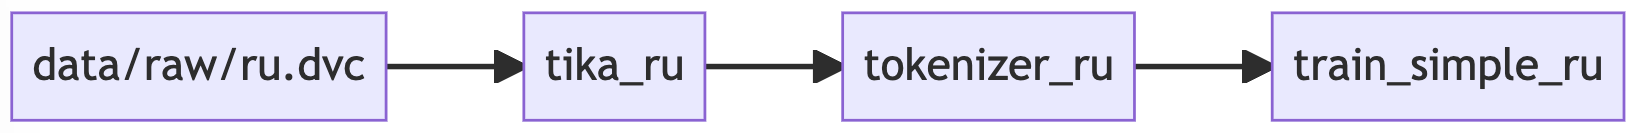
\includegraphics[width=\linewidth]{dvc-pipeline}
    \caption{Визуальное представление \acrshort{dag} обучения}
    \label{fig:dvc-pipeline}
\end{figure}

Приведенный на рисунке \ref{fig:dvc-pipeline} граф был построен по следующим правилам:
\begin{enumerate}
    \item Каждая стадия и каждый явно прописанный входной файл представляются вершинами графа.
    \item Для каждой стадии анализируется список ее зависимостей (\textit{deps}).
        Если эти зависимости удовлетворяются одной из описанных стадий (проверются выходные файлы стадии) или входным файлом, указанном наравне со стадиями, то проводится ребро между двумя стадиями, направленное в стороне зависимой.
        Если зависимости не удовлетворяются, то выдается ошибка запуска.
    \item Проверяется наличие циклов в полученном графе.
        Если они обнаружены, то выдается ошибка запуска.
\end{enumerate}
Построенный таким образом граф не только задает последовательность операций, но и явно описывает все входные и выходные данные.
Это позволяет настроить \textit{статистические проверки на наличие данных}, которые описаны среди проблем в \ref{sec:ml-debt}.
Помимо этого, описание всего процесса в едином графе вычислений дает возможность управлять процессом и производить его масштабирование, добавляя тем самым \textit{способность к управлению множественными процессами}.

Помимо выстраивания \gls{pipeline}, \gls{dvc} предоставляет широкий спектр других возможности для автоматизации задач машинного обучения.
К примеру, возможно создавать так называемые <<эксперименты>>, которые представляют из себя воспроизводимый запуск всего \gls{pipeline} с измениями в конфигурации и/или исходном коде моделей.
Помимо этого поддерживается экспериментальная поддержка работы на удаленной машине (см. документацию \cite{cite:dvc}).
При таком подходе компьютер разработчика выступает в роли т.н. тонкого клиента -- весь код редактируется локально, а фактические вычисления осуществляются на удаленном компьютере.

Разделение кода на стадии, предлагаемое в \gls{dvc}, позволяет выстроить четкое разделение процесса на состоявляющие компоненты, избавляя от описанной в \ref{sec:ml-debt} проблемы <<спагетти>>-кода: вместо единого большого файла с набором инструкций будет порождено несколько небольших скриптов, выполняющих одну задачу, и выполняющих ее хорошо.
В настоящей работе удалось успешно осуществить такое разделение.
Первональная версия модели, выполненная в едином файле \gls{jupyter-notebook}, была разбита на множество отдельных скриптов, каждый из которых расширял и обобщал существующую функциональность исходного прототипа.
\section{Версионирование данных, артефактов и визуализация метрик}
\label{sec:dvc}
% TODO: (ruapyyj) ну, тоже dvc <- Tue Apr 26 23:11:29 2022

\subsection{Проблемы при версионировании данных}
\label{sec:dvc-versioning-problems}
С теоретической точки зрения версионирование данных ничем не отличается от версионирования исходного кода.
Ожидается, что система хранения данных способна возвращаться к любой заранее отмеченной версии, хранить эти версии в удаленном хранилище и иметь возможность переключаться между различными версиями.
Практическая реализация, тем не менее, осложняется по нескольким причинам.

Во-первых, существующие системы контроля версий (\acrlong{vcs}) изначально создавались для хранения файлов исходного кода, имеющих малый размер, что в большинстве случаев определило их архитектуру.
Так, используемый в данной работе \gls{git} по умолчанию выгружает полную копию всех версий всех файлов, находящихся под отслеживанием, что не является проблемой для <<легких>> файлов (например, небольших документов, исходного кода), но совершенно неприменимо для больших файлов с данными, используемых в \acrshort{ml}-проектах.

Вторая причина состоит в том, что большинство \acrshort{vcs} реализуют собственные системы для физического хранения версий объектов -- к примеру, \gls{git} сохраняет файлы в директории \texttt{.git/}, полученной от сервера с исходными кодами.
Собственные реализации хранилища могут быть применимы и для данных большего размера, но зачастую под хранение объектов значительного объема используются специализированные под такую задачу решения (например, \gls{s3}-хранилища, система \gls{hadoop} с ее распределенной файловой системой \gls{hdfs} и т.п.).

Описанные проблемы решены в \gls{dvc}.
Вместо версионирования самих файлов с данными \gls{dvc} отправляет в \acrshort{vcs} файл с хеш-суммой файла (по умолчанию используется MD5).
Сам файл отправляется в кэш (может храниться как локально, так и на \gls{hdfs}).
Каждая версия файла таким образом будет представлять из себя пару (\textit{файл с хешом}, \textit{файл с содержимым}), где последний исключается из отслеживания \gls{vcs}.
Когда необходимо переключиться между версиями, соответствующий хеш-сумме файл достается из кэша и перекладывается в рабочую область.

Кэш с файлами допускает хранение на удаленных серверах.
В \gls{dvc} реализована поддержка большого количества хранилищ: \acrshort{sshfs}, \gls{hdfs}, \gls{s3}, \gls{webdav} и других (полный список доступен в \href{https://dvc.org/doc/command-reference/remote/add#supported-storage-types}{документации}).
Такой подход позволяет использовать уже существующую инфраструктуру для задач версионирования.

\subsection{Решение в рамках данной работы}
В \ref{sec:dvc-pipeline} было указано, что каждая стадия имеет явно заданные входные и выходные данные.
Помимо \textit{наблюдаемости} данных (возможности в любой момент знать, какие данные для чего используются) это позволяет вести их учет, версионировать и сохранять в надежных хранилищах (например, в \gls{s3}).
Описанная возможность успешно реализована в настоящей работе силами фреймворка \gls{dvc}.

Вход и выход каждой стадии версионируется упомянутым фреймворком в соответствии с процедурой, описанной в \ref{sec:dvc-versioning-problems}.
Кэш объектов хранится локально на диске большого объема и на удаленном \gls{s3}-хранилище (в целях обеспечения отказоустойчивости).

Подобная организация позволяет решить несколько проблем из \ref{sec:ml-debt}.
Во-первых, все зависимости от данных становятся \textit{стабильными} за счет того, чтобы данные версионируются, имеют привязку к версии кода (\gls{dvc} достигает это через добавление файла с хешом в \gls{vcs}) и надежно хранятся в удаленном хранилище.

Во-вторых, появляется \textit{воспроизводимость} процесса -- каждый разработчик в состоянии запустить весь \gls{pipeline} с теми же входными данными и версиями кода, что и были в прошлых запусках.
Здесь стоит заметить, что для \textit{полной воспроизводимости} необходимо также убедиться, что каждый скрипт при одинаковых входных данных будет производить одинаковые выходы от запуска к запуску.
В настоящей работе это было достигнуто фиксированием random seed и значения текущего времени во всех зависимых от времени в инструкциях (подробнее о техниках воспроизводимости описано в \cite{cite:ml-reproducibility}).

В-третьих, указание файла настроек в качестве зависимости привело к \textit{отслеживанию конфигурации} всего \gls{pipeline} и автоматическому перерасчету релеватных стадий при изменениях в настройках.
Для получения всех преимуществ подобного отслеживания в настоящей работе все настройки всего \gls{pipeline} обучения (кроме сбора данных краулерами) были вынесены в единый файл (концепция <<single source of truth>>).
Этот файл версионируется, используя \gls{git}, и изменения в нем служат индикатором для перезапуска тех стадий, которые зависят от измененных параметров.

Стадия обучения модели настроена на выгрузку весов и внутренней структуры леса в отдельные файлы, каждый из которых прописан в настройках \gls{dvc} -- благодаря этому артефакты обучения подлежат версионированию и хранению наравне с данными.

\subsection{Визуализация в \gls{dvc}}
Особое внимание стоит обратить на работу с метриками и графиками.
\Gls{dvc} позволяет не только версионировать метрики и данные для графиков, но и сравнивать их между различными ревизиями.

Для сравнения метрик между собой их необходимо выгрузить в файл в одном из поддерживаемых форматов (в работе используется \texttt{JSON}) и описать файл в \gls{dvc} \gls{pipeline}.
После этого появится возможность сравнивать различные версии этого файла между собой и строить отчеты в формате Markdown.
Такое сравнение удобно, когда требуется быстро понять результат тех или иных изменений в коде или данных.
Формат метрик никак не ограничивается -- возможно хранить любые JSON-сериализуемые пары <<ключ-значение>>.
Пример отчета по метрикам со сравнением между ревизиями показан в таблице \ref{table:dvc-metrics-diff}.

\begin{table}[!ht]
    \centering
    \begin{tabular}{|l|l|l|l|l|}
    \hline
        Path & Metric & main & 0b257f19 & Change \\ \hline
        it/metrics.json & Businises\&Corporate.f1-score & 0.96526 & 0.96487 & -0.00039 \\ \hline
        it/metrics.json & Businises\&Corporate.precision & 0.96487 & 0.96412 & -0.00075 \\ \hline
        it/metrics.json & Businises\&Corporate.recall & 0.96566 & 0.96562 & -3e-05 \\ \hline
        it/metrics.json & Businises\&Corporate.support & 1223 & 1280 & 57 \\ \hline
        it/metrics.json & Finance\&Banking.f1-score & 0.99403 & 0.99379 & -0.00023 \\ \hline
        it/metrics.json & Finance\&Banking.precision & 0.99289 & 0.99346 & 0.00057 \\ \hline
        it/metrics.json & Finance\&Banking.recall & 0.99517 & 0.99413 & -0.00104 \\ \hline
        it/metrics.json & Finance\&Banking.support & 4347 & 4430 & 83 \\ \hline
    \end{tabular}
    \caption{Пример сравнения метрик между ревизиями}
    \label{table:dvc-metrics-diff}
\end{table}

\begin{figure}[!h]
    \centering
    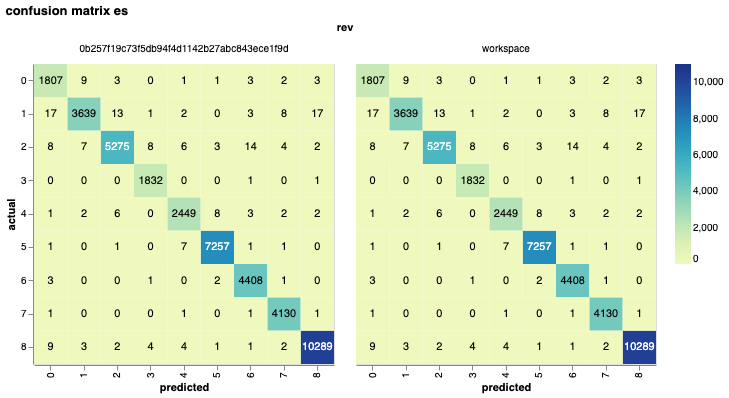
\includegraphics[width=\linewidth]{dvc-plots-diff}
    \caption{Пример сравнения confusion matrix между ревизиями. В заголовке каждого графика указывается ревизия, по которой тот был отрисован. Метки классов представлены числами.}
    \label{fig:dvc-plots-diff}
\end{figure}
\begin{figure}[!ht]
    \centering
    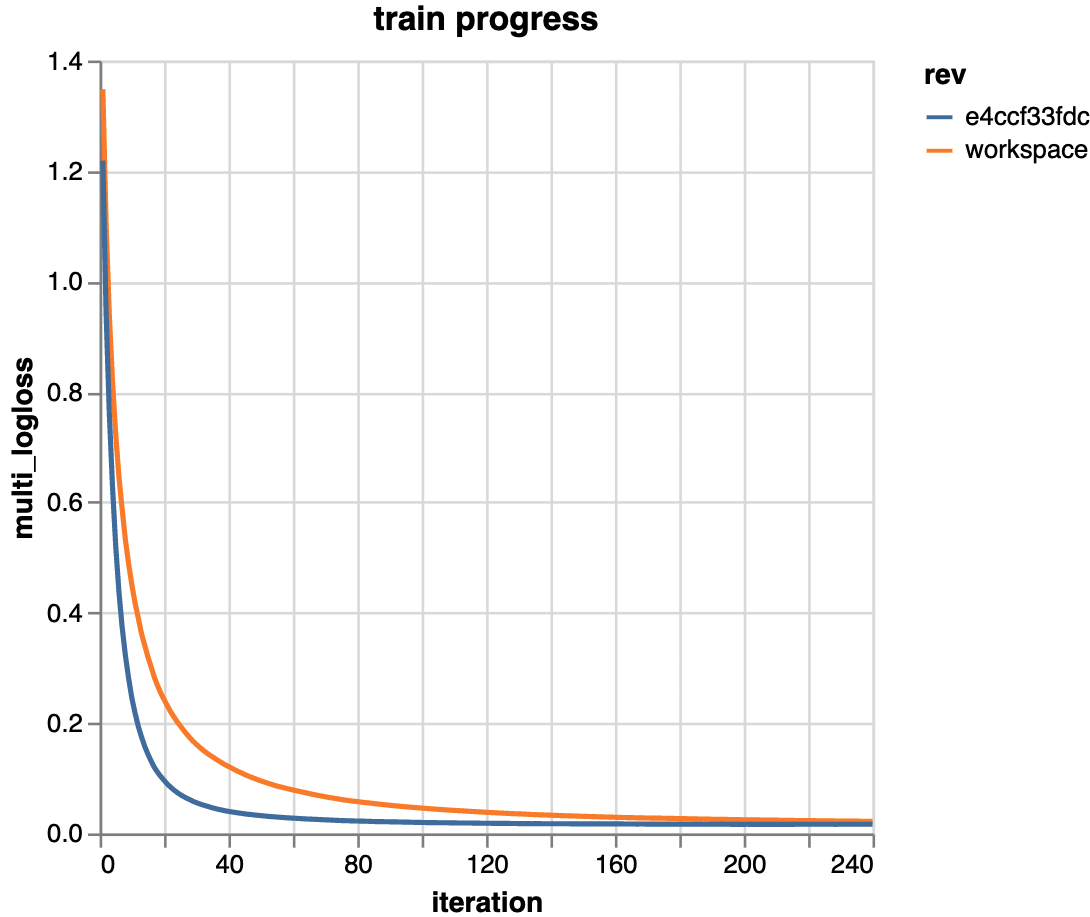
\includegraphics[width=0.9\linewidth]{dvc-plots-diff-real}
    \caption{Пример отображения различий в графиках между ревизиями}
    \label{fig:dvc-plots-diff-real}
\end{figure}
В случае графиков имеется аналогичная возможность сравнения ревизий.
Требуется выгрузить данные для построения графиков в отдельный файл, описать его в \gls{dvc} \gls{pipeline}, после чего появится возможность отрисовки графиков двух версий на одном полотне.
Пример этого представлен на рис. \ref{fig:dvc-plots-diff}.

При отрисовке кривых обе отображаются на одном графике для простоты визуального сравнения -- как это показано на рисунке \ref{fig:dvc-plots-diff-real}.

На рисунке \ref{fig:dvc-plots-labels} можно видеть confusion matrix с текстовым указанием классов.
\begin{figure}[!ht]
    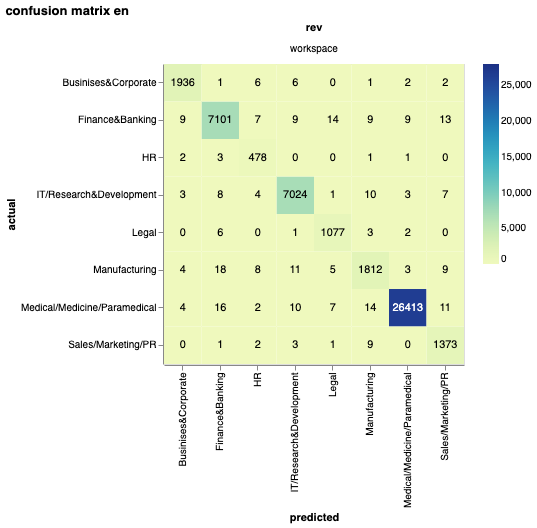
\includegraphics[width=\linewidth]{dvc-plots-labels}
    \caption{Пример confusion matrix с текстовым указанием классов}
    \label{fig:dvc-plots-labels}
\end{figure}

Существует веб-сайт, в котором возможно получать все упомянутые визуализации в режиме онлайн.
Это DVC Studio, продукт от создателей \gls{dvc}.
Проект, описываемый в настоящей работе, можно найти \href{https://studio.iterative.ai/user/alekseik1/views/dataclassification-crawler-e1vtfsj7dv}{здесь}, а на рисунке \ref{fig:studio} изображен пример работы с сайтом.

\begin{figure}[!h]
    \centering
    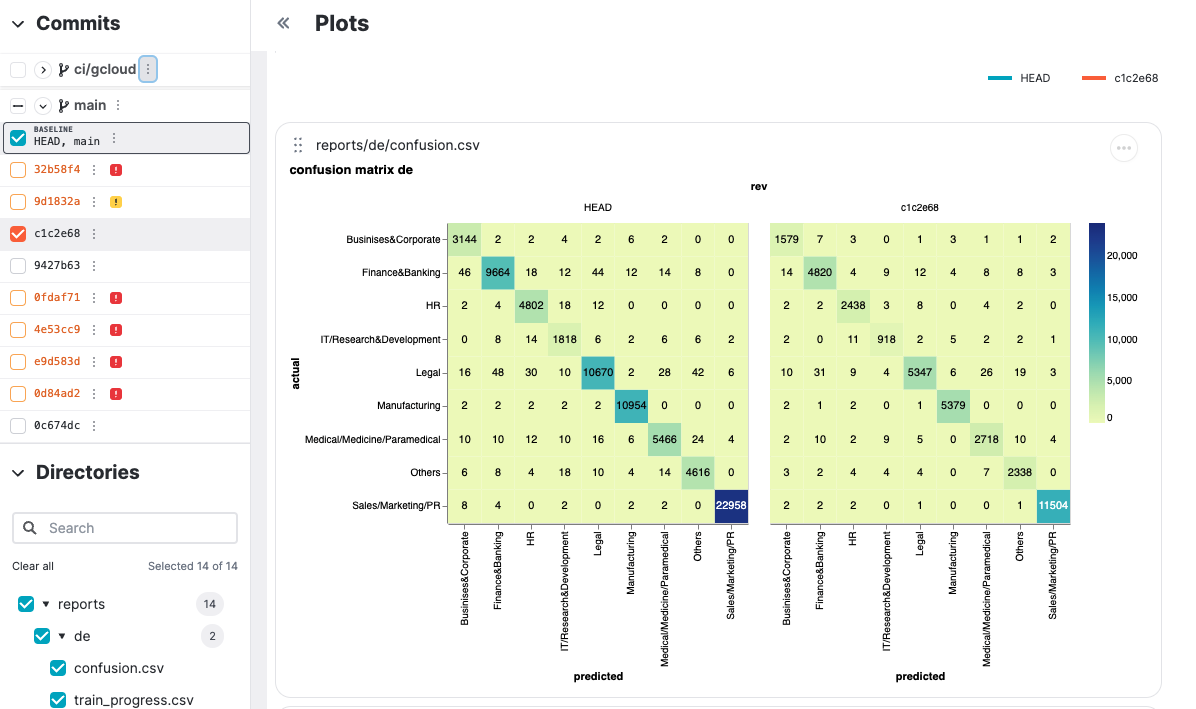
\includegraphics[width=\linewidth]{studio}
    \caption{Интерфейс веб-страницы с визуализацией метрик}
    \label{fig:studio}
\end{figure}
\section{Журналирование, хранение старых экспериментов}
Из описанных в \ref{sec:ml-debt} проблем остаются \textit{тупиковых экспериментальных ветвлений} и \textit{мониторинга с журналированием}.
Первая из них решена в данной работе использованием тегов в \gls{git} -- на каждый эксперимент выставляется тег, но изменения кода модели не вливаются в основную ветку при отсутствии успеха.
В таком случае основная ветка остается свободной от остатков неудачных экспериментов и тупиковых условных переходов внутри кода.
К неудавшемуся эксперименту всегда будет возможно вернуться, поскольку использованные в нем данные и код версионируются \gls{dvc}.

Вторая проблема решена частично -- в код модели встроено обильное логгирование.
Логи складируются в файлы, разделенные отдельными запусками, и каждая запись имеет унифицированный формат, что облегчит последующую обработку автоматическими инструментами по работе с журналами.
Примеры таких инструментов приведены в секции \ref{sec:future}.

Хранение старых экспериментов реализовано силами \gls{dvc}.
Встроенная в этот инструмент возможность хранить артефакты каждой стадии \gls{pipeline} с привязкой к коммиту \gls{git} активно используется в настоящей работе.
А использование \gls{s3}-хранилища дает возможность надежно хранить артефакты любой версии.

Таким образом, использование в данной работе \gls{dvc} и продвинутых возможностей \gls{git} позволило решить все проблемы, намеченные в \ref{sec:ml-debt}.
Подкрепленная такими возможностями, построенная на одной локализации модель допустила обобщение, в результате чего удалось автоматизировать процесс обучения на новых данных, обобщить его на другие языки и упростить процесс коллаборации с другими участниками проекта.
\section{Дальнейшие планы по работе}
\label{sec:future}
Проведенные в настоящей работе усилия по автоматизации значительно приблизили первоначальный прототип системы классификации документов к состоянию самообучаещейся модели.
Тем не менее, возможны дальнейшие улучшения, намеченные к реализации в будущей работе.
Ниже кратко рассмотрены планы по дальнейшей работе.
    \subsection{Выстроение обучения в \gls{cicd}}
    Предполагается выполнять тестовый запуск всего пайплайна обучения на сервере при каждом успешном Merge Request в основную ветку, как показано на \ref{fig:cicd}.
    \begin{figure}[h]
        \centering
        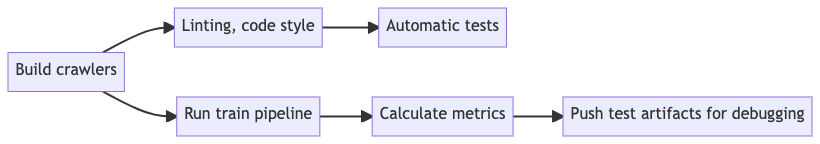
\includegraphics[width=\linewidth]{cicd}
        \caption{Предполагаемая настройка \gls{cicd} пайплайна}
        \label{fig:cicd}
    \end{figure}
    На остальных ветках \gls{pipeline} обучения будет выполняться над небольшим набором данных, чтобы быстрее получить и передать разработчикам обратную связь.
    Это позволит ускорить итерации разработки и автоматизировать переобучение при обновлении кодовой базы.

    Для реализации такой задачи хорошо подойдет инструмент \href{https://cml.dev/}{CML}
    \subsection{Валидация входных данных при обучении}
    При обучении модели имеет смысл исключать выбросы, поскольку ее качество может значительно пострадать при наличии существенных отклонений в данных.
    Разработка алгоритма определения неподходящих для обучения данных и последующая автоматизация этого алгоритма позволит увеличить метрики качества модели без существенного изменения ее сути.
    \subsection{Автоматическое детектирование серьезных отклонений в предсказаниях}
    Текущая реализация модели может предсказывать вероятность каждого из классов.
    Имеет смысл сохранять те документы, на которых модель имеет близкие вероятности у двух различных классов -- документы, в которых модель <<не уверена>> в предсказаниях.
    Впоследствии такие примеры следует проанализировать, дабы извлечь закономерность появления неоднозначности ответа модели.

    Предположительно данная задача может быть решена с использованием инструмента от \href{https://evidentlyai.com/}{evidently AI}.
    \subsection{Улучшение ручной разметки входных данных}
    На этапе прототипирования был выбран очень простой алгоритм разметки: если сайт имеет тематику $X$, то всего документы помечаются как имеющие тематику $X$.
    Такая разметка проста в реализации, но не является до конца корректной -- поэтому ее улучшение может повысить качество модели.

    Среди возможных способов стоит отметить применение кластеризации документов, размечивание с привлечением экспертов и использование более сложных моделей (или ансамблей) для исключения ошибок текущей разметки.
    \subsection{Централизованная система логгирования}
    Хранение и анализ логов полезно для работы над ошибками в программе и поиска узких мест всего процесса.
    По мере роста проекта количество журналов значительно растет, и возникает нужда в автоматических средствах хранения, поиска и обработки логов.
    На момент написания работы логи каждого шага всего процесса обучения пишутся в файлы, хранимые локально на сервере запуска (описанном в приложении \ref{sec:gcloud}).

    Для решения такой проблемы можно использовать одно из готовых решений -- к примеру, стек \gls{elk} или его простой аналог \href{https://www.graylog.org/}{Graylog}.
